\clearpage
\chapter{Serial communication protocols} \label{Basics_motor_control}

\section{UART (Universal Asynchronous Receiver/Transmitter)}

\begin{figure}[h!]
\centering
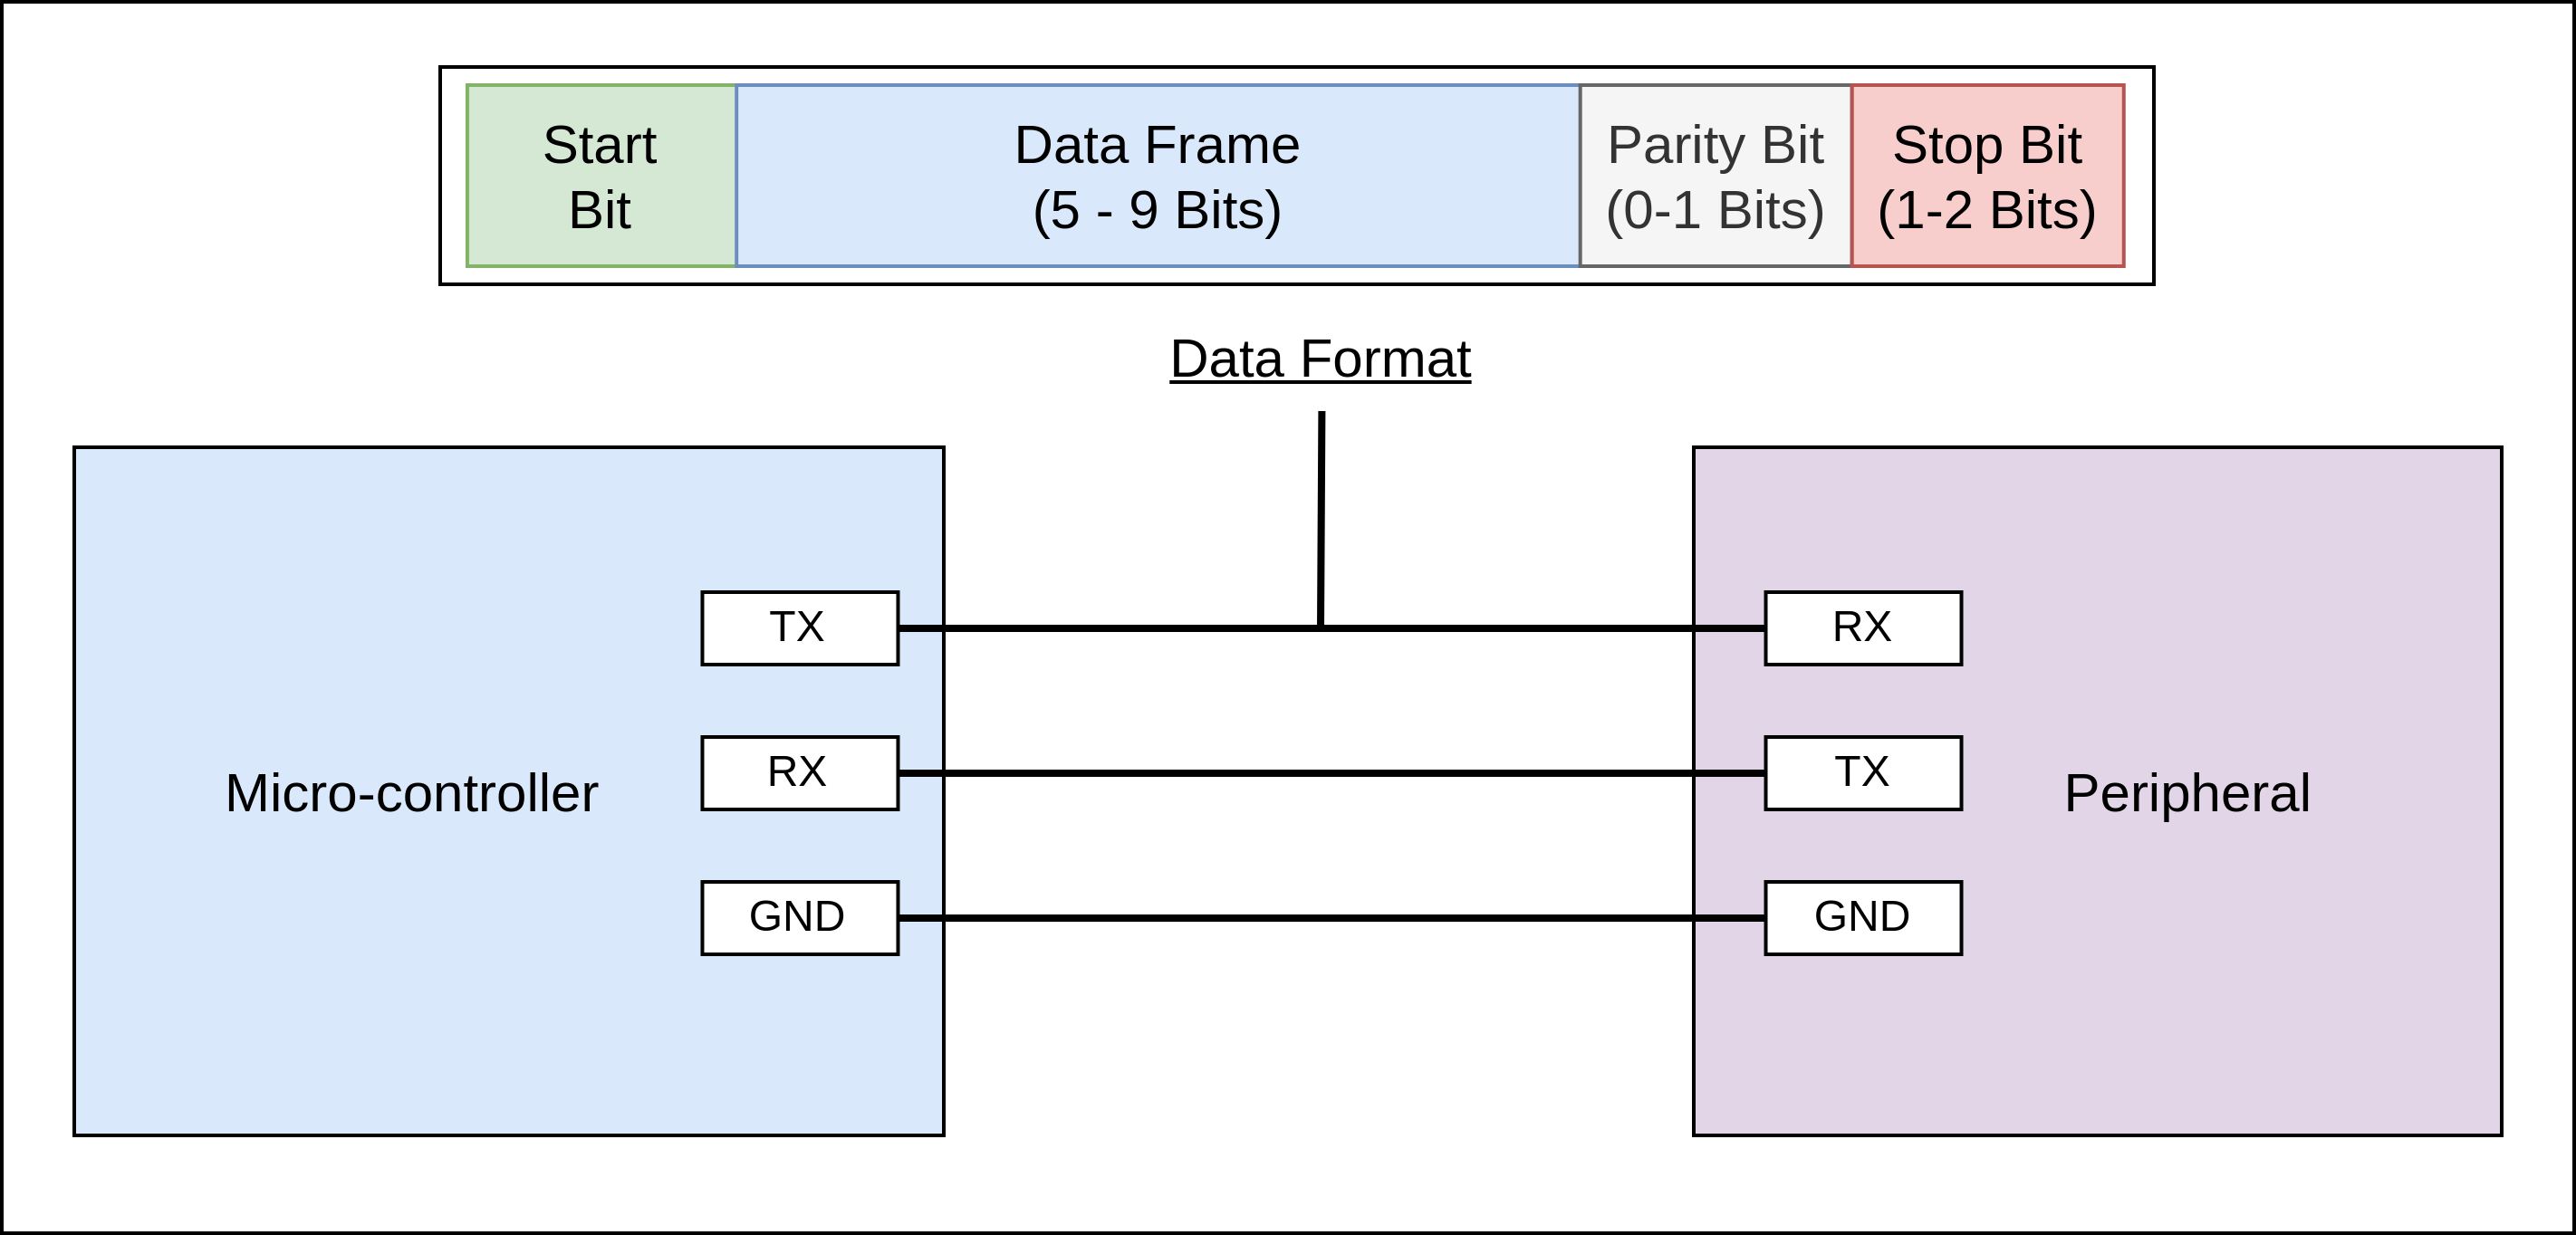
\includegraphics[width=14cm]{./Figures/UART.png}
\caption{Data format and connection between two devices in UART interface}
\label{UART}
\end{figure}

Features of UART interface:
\begin{itemize}
    \item UART is a lower data serial communication protocol. The receiver device should know baud-rate of the transmitter device before actual communication establishment.
    \item UART is simple protocol, it uses start bit (before data word), stop bits (one or two, after data word), parity bit (even or odd) in its base format for data formatting. Parity bit helps in one bit error detection. UART Packet = 1 start bit(low level), 8 data bits including parity bit, 1 or 2 stop bit(high level)
    \item Data is transmitted byte by byte. UART does not have clock as it is asynchronous serial communication protocol. It makes use of stop and start bits to synchronise the communication process. For long distance communication, 5V UART is converted to higher voltages viz. +12V for logic 0 and -12V for logic 1. The figure \ref{UART} below shows UART interface between two devices.
    
    
\end{itemize}

\section{SPI (Serial Peripheral Interface)}
\begin{itemize}
    \begin{figure}[h!]
    \centering
    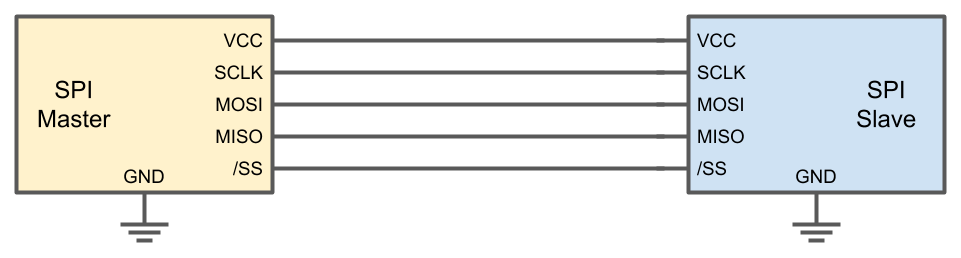
\includegraphics[width=11cm]{./Figures/SPI_single_slave.png}
    \caption{SPI point-to-point connections}
    \label{SPI_single_slave}
    \end{figure}
    \item SPI is a protocol on 4 signal lines:
    \begin{itemize}
        \item A clock signal named SCLK, sent from the bus master to all slaves; all the SPI signals are synchronous to this clock signal;
        \item A slave select signal for each slave, SSn, used to select the slave the master communicates with;
        \item A data line from the master to the slaves, named MOSI (Master Out-Slave In)
        \item A data line from the slaves to the master, named MISO (Master In-Slave Out)
    \end{itemize}
    \item Two SPI bus Topologies:
    \begin{itemize}
        \item SPI Master connected to a single slave (Point-to-Point topology) as shown in figure \ref{SPI_single_slave}.
        \item SPI Master connected to multiple slaves as shown in Figure \ref{SPI_multi_slave}.
    \end{itemize}
    \begin{figure}[h!]
    \centering
    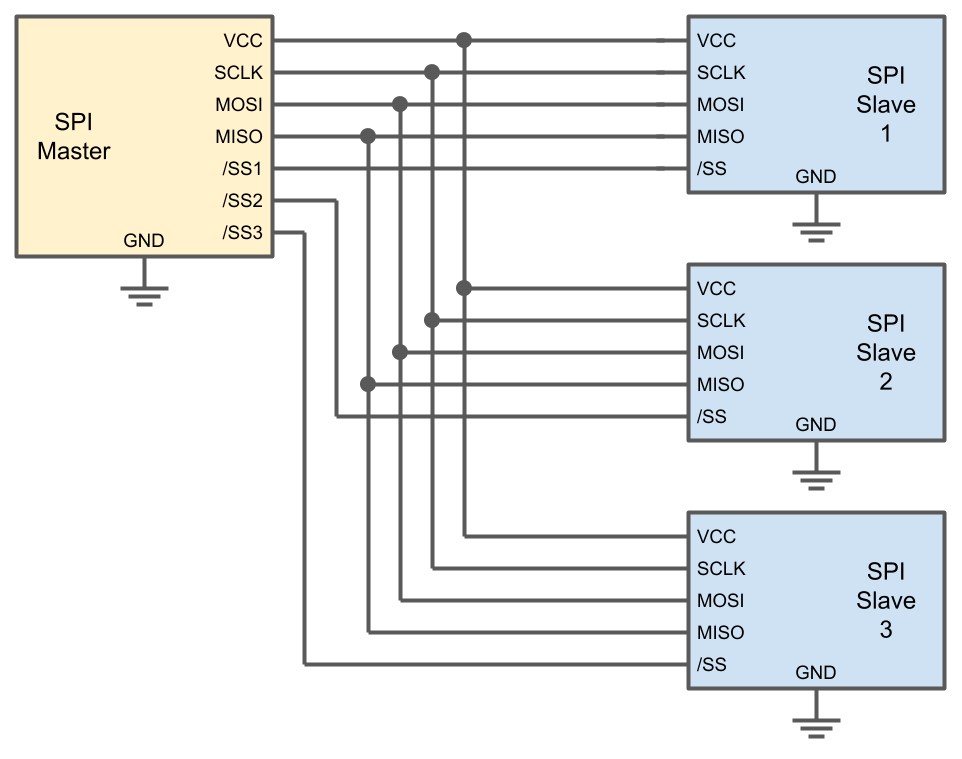
\includegraphics[width=11cm]{./Figures/SPI_multi_slave.png}
    \caption{SPI connections for 3 slave devices}
    \label{SPI_multi_slave}
    \end{figure}
\end{itemize}

\newpage
\section{I2C Protocol}

\begin{figure}[h!]
\centering
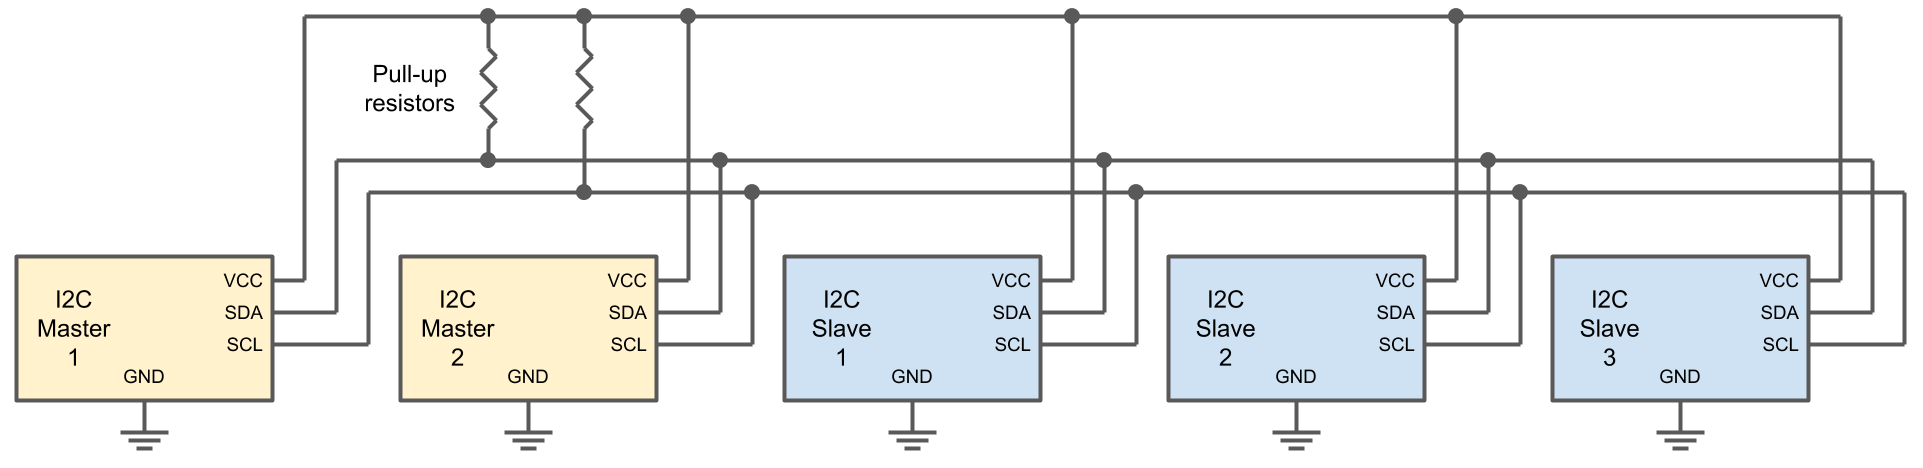
\includegraphics[width=\columnwidth]{./Figures/I2C_multi_master.png}
\caption{I2C connections for multiple master and multiple slave devices}
\label{I2C_multi_master}
\end{figure}

Features:
\begin{itemize}
    \item I2C is a two-wire communication protocol that is commonly used to connect low-speed devices like micro-controllers, I/O interfaces, A/D and D/A converters, EEPROMs, and other peripherals in embedded systems.
    \item One of these wires, known as SCL (Serial Clock) carries the clock signal, while the other wire, known as SDA (Serial Data) allows master and slave devices on the bus to send and receive data. The I2C protocol allows for multiple slave devices to be connected to a single master device, or for multiple masters controlling one or more slave devices (Figure \ref{I2C_multi_master}).
\end{itemize}